\documentclass[12pt,a4paper]{article}
\usepackage[utf8]{inputenc}
\usepackage[brazil]{babel}
\usepackage{graphicx}
\usepackage{amssymb, amsfonts, amsmath}
\usepackage{float}
\usepackage{enumerate}
\usepackage[top=1.5cm, bottom=1.5cm, left=1.25cm, right=1.25cm]{geometry}

\begin{document}
\pagestyle{empty}

\begin{center}
  \begin{tabular}{ccc}
    \begin{tabular}{c}
      
\includegraphics[scale=0.25]{../../biblioteca/imagem/brasao-de-armas-brasil} \\
    \end{tabular} & 
    \begin{tabular}{c}
      Ministério da Educação \\
      Universidade Federal dos Vales do Jequitinhonha e Mucuri \\
      Faculdade de Ciências Sociais, Aplicadas e Exatas - FACSAE \\
      Departamento de Ciências Exatas - DCEX \\
      Disciplina: Matemática Elementar I \quad Semestre: 2021/1\\
      Prof. Me. Luiz C. M. de Aquino\\
    \end{tabular} &
    \begin{tabular}{c}
      
\includegraphics[scale=0.25]{../../biblioteca/imagem/logo-ufvjm} \\
    \end{tabular}
  \end{tabular}
\end{center}

\begin{center}
 \textbf{Avaliação II}
\end{center}

\textbf{Instruções}
\begin{itemize}
 \item Todas as justificativas necessárias na solução de cada questão devem estar presentes nesta avaliação;
 \item As respostas finais de cada questão devem estar escritas de caneta;
 \item Esta avaliação tem um total de 35,0 pontos.
\end{itemize}

\begin{enumerate}
  \item \textbf{[7,0 pontos]} Determine a função $f$ polinomial do 1° grau tal que seu gráfico passa
  pelos pontos $(-2,\,-6)$ e $(12,\,1)$.

  \item \textbf{[7,0 pontos]} Em certa loja de calçados os vendedores recebem de salário 
  um valor fixo de R\$ 1.600,00 e mais uma comissão de 3,5\% sobre o total de
  vendas que eles efetuarem no mês. Se em certo mês um vendedor recebeu
  R\$ 2.704,60 de salário, então qual foi o total de vendas dele nesse mês?

  \item \textbf{[7,0 pontos]} Determine a função $f$ polinomial do 2° grau tal que seu gráfico passa
  pelos pontos $(0,\,0)$, $(5,\,6)$ e $(10,\,10)$.

  \item \textbf{[7,0 pontos]} Determine a função $f$ polinomial do 2° grau tal que $f(0) + f(1) = -1$,
    $f(2) = f(-2)$ e $f(-1) = 0$.

  \item \textbf{[7,0 pontos]} Considere que $f$ é uma função polinomial do 2° grau, cujo o gráfico está
  ilustrado abaixo. Determine os pontos que esse gráfico corta o eixo $x$.

  \begin{figure}[H]
   \centering
   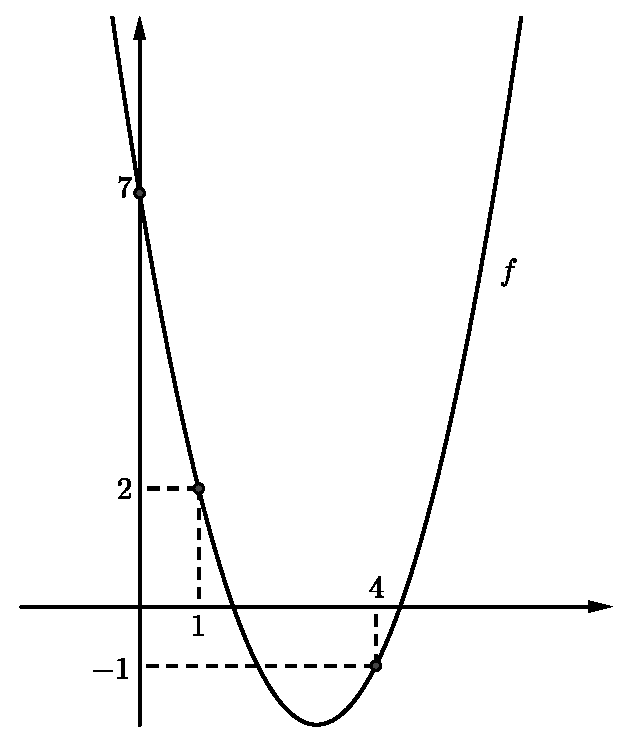
\includegraphics[scale=0.625]{figura/grafico-funcao-polinomio-segundo-grau.eps}
  \end{figure}

\end{enumerate}

\end{document}